\newcommand{\Cont}{\mathcal{C}}%
%
% Introduction of the necessity of reduction of an abstraction
Graph search algorithm complexities are dependant on the size of the abstraction.
These methods suffer from the state space explosion problem: the complexity of graph search algorithm have usually an exponential complexity in the size of the state space.

% Property that needs to be verified by the abstraction
Therefore it is of a great interest to design small abstractions for the controller synthesis.
The new abstraction needs to verify alternating similarity relationship with the original abstraction.

\section{Related work}
Talk about formal verifications methods.

The needs of discrete abstraction.

%% MOVE THIS PART
In \cite{tabuada2009verification}, the link between in hybrid systems is investigated. 
\begin{nameddef}{System}
$\mathcal{T}_c = (X,X_0,U, \transition, Y,H)$
where:
\begin{itemize}[noitemsep,nolistsep]
\item $X$ is a set of states;
\item $X_0 \subset X$ a set of initial states;
\item $U$ a set of inputs;
\item $\transition \subseteq X \times U \times X$ a transition relation ;
\item $Y$ a set of outputs;
\item $H:X \rightarrow Y$ an output map.\popQED
\end{itemize}
\end{nameddef}

The alternating simulation relation between 2 systems is the link between discrete abstraction and the continuous representation of this system.
For comoditiy, the definition of alternative simulation is rewritten here (\cite{tabuada2009verification}):
\begin{nameddef}{Alternating simulation} \label{def_alt_sim}
Let $\sysA$ and $\sysB$ 2 systems with $Y_a=Y_b$, $\sysA$ is alternatingly simulated by $\sysB$ if there exists a relation $R \subseteq X_a \times X_b$ that verify:
\begin{enumerate}[noitemsep,nolistsep]
\item $\forall x_{a0} \in X_{a0}, \exists x_{b0} \in X_{b0}, (x_{a0},x_{b0}) \in R$
\item $\forall (x_a,x_b) \in R, H_a(x_a) = H_b(x_b)$
\item $\forall (x_a,x_b) \in R, \forall u_{a} \in U_{a}, \exists u_{b} \in U_{b}$\\
$\forall x_b' \in Post_{u_b}(x_b),\exists x_a' \in Post_{u_a}(x_a), (x_a',x_b') \in R$
\popQED
\end{enumerate}
\end{nameddef}
The alternating simulation relation between $\sysA$ and $\sysB$ is weaker than the bisimulation relation (that require the alternating simulation relation between $\sysA$ and $\sysB$ and between $\sysB$ and $\sysA$).

Lets denote the composition of systems by the operator $\times$.
If $sysA$ alternatingly simulate by $\sysB$ for a controller $\Cont$ composable with $\sysA$ or $\sysB$, then $\sysA \times \Cont$ verify the same reachability properties than $\sysB \times \Cont$, and $\sysB \times \Cont$ verify the same safety properties than $\sysA \times \Cont$.

\section{Abstraction reduction}
Our approach in order to reduce the size of an abstraction $\sys$ is create an abstraction $\sysa$ with a smaller state space than $\sys$ and to add the knowledge of the last $\Ninputs$ inputs of the system.

The term "reduction" will be justified later. This does not always correspond to a reduction of the abstraction size (the set of all the input sequences might be larger than the size of the states dimensions that have be suppressed). However, the efficient utilization of this methods correspond to a reduction of the state space size.

% Describe how it is done
To use control synthesis methods with the new abstraction $\sysa$, we need that $\sys$ and $\sysa$ have an alternating simulation relation.

Without loss of generality, lets assume that the state $\x$ of the system $\sys$ can be decomposed in this way $\x = [\xobs,\xunobs]$ where $\xobs$ is observed and $\xunobs$ is an unobserved (internal) state.
In practice, the state $\xunobs$ correspond to the part of the system that we will suppress.
Then the states of $\sysa$ will be expressed by $\xa_n = [\xobs_n,\Pastuseq]$ where $\Pastuseq = [\pastuseq]$ correspond to the $\Ninputs$ last control actions.

%% TODO: I REALLY NEED TO IMPROVE THE EXPLAINATION AT THE BEGGINNING
In order to compute the successors of the the state $\xa_n$, we need to find the set $\Xunobs(\Pastuseq)$ of all the possible states $\xunobs_n$ of system $\sys$ after applying the control sequence $\Pastuseq$.
This problem is a reachability problem.
It can be solved in 2 steps: find the smallest invariant $\Xuinv$ of $\sys$ dynamics on $\xunobs$; compute $\Xunobs(\Pastuseq)$ the image of $\Xuinv$ after applying the sequence $\Pastuseq$.

% Definition of the reduced system
Let the system
$\sysa =  (X_a,X_{a 0}, \sysaU, \transition, Y_a, H_a)$ 
where 
$X_a = \Xobs \times \sysaU^{\Ninputs}$ the set of states, 
$X_{a 0} = \Xobsinit \times  \mathcal{U}^{\Ninputs}$ the set of initial states, 
$Y_a = \Xobs$ the set of outputs
and the output map $H_a$ that correspond to the projection from $X_a$ on $\Xobs$.
The transition relation is defined by:
\begin{equation}
\begin{split}
(\xobs_n,\vect{u}_{n - \Ninputs},...,\vect{u}_{n-1}) 
\labelledtransition{\vect{u}_n} 
& (\xobs_{n+1},\vect{u}_{n+1-\Ninputs},...,\vect{u}_{n-1},\vect{u}_n)\\ \Longleftrightarrow 
\xobs_{n+1} \in 
& H_a(Post^S_{u}(\{\xobs\} \times \Xunobs(\vect{u}_{n - \Ninputs},...,\vect{u}_{n-1}))
\end{split}
\end{equation}

\begin{figure}
\centering
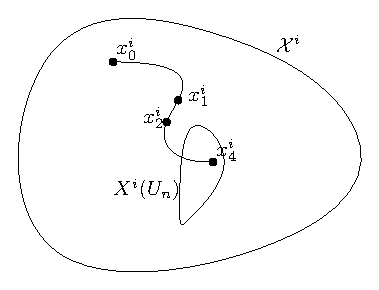
\includegraphics[width=0.5\linewidth]{invariant_set}
\caption{The image of the invariant set $\Xuinv$ after applying the control sequence $\Pastuseq$ is $\Xunobs(\Pastuseq)$}
\end{figure}

%% MISSING PROOF THAT IT IS AN ALTERNATING SIMULATION RELATION
\begin{prop}
$\sys$ is alternately simulated by $\sysa$.
\end{prop}

\begin{proof}
Lets take the relation $R$ defined by:
\begin{equation}
R = \{ (\x,\xa) \in X \times X_a \mid H(\x) = H_a(\xa) \}
\end{equation}
By definition of the systems $\sys$ and $\sysa$ and of the relation $R$, conditions \ref{def_alt_sim}.1 and \ref{def_alt_sim}.2 are verified.

In order to prove that condition \ref{def_alt_sim}.3 lie, it is sufficient to show that the unobserved part of $\x$ is contained in the set $\Xunobs(\Pastuseq)$.
\end{proof}

By construction, $S_a$ is an alternating simulation relation of the the system $S$.
\textit{PS: I need to prove that the state of $S$ are staying in $X^z \times X^\infty_r$.}

If the dynamics of $\sys$ on $\xunobs$ have a bounded effect of the rest of the system 
If the states $\xunobs$ of $S$ are unstable, this estimation is not possible.

Our goal is estimate the set $\Xunobs$ of all the possible state $\xunobs$ after applying the sequence $[\pastuseq]$ of controls.

% where do I talk about the stability properties?
% what do I need to say about it? Does it needs to be proved

% Conditions about the stability of the system
The sequence of inputs will be used to compute the reached set of $\xunobs$.

% Linear system, I need it there mainly because for the alternating simulation relation, I need the decouppling property. It is easier to use LTI for this.
From now we will use linear time invariant systems. We use them mainly for their ease of manipulation.

\section{Influence of control sequences}
In this part we will try find an alternating simulation relation between a linear system that verify some properties with a new system where we don't observe all the states but we know the last $\Ninputs$ controls that we used.

We aim to reduce the complexity of the problem.

\begin{problem}
Find an alternating simulation relation on the space with inputs that minimize the number of successors for each nodes.
\end{problem}

To do this we need several assumptions: the states that we are going to suppress must behave in a good way (asymptotically stable).
We will have to bound the effect of the suppressed dynamic, this mean also that any other components (inputs, noise and other states) must have a bounded effect on these dynamics.

